\documentclass[a4paper,11pt]{article}

%%%%%%%%%
%%usees%%
%%%%%%%%%
\usepackage[utf8]{inputenc}
%\usepackage[ngerman]{babel}
%\usepackage{a4wide}
\usepackage[margin=3.0cm, top=3.0cm, bottom=3.0cm]{geometry}
\usepackage{setspace}
\usepackage{graphicx}
\usepackage{amssymb} 
\usepackage{amsmath}
\usepackage{mathtools}
\usepackage{footnote}
\usepackage{caption}
\usepackage{color}
\usepackage[hidelinks]{hyperref}
\usepackage{cite}
\usepackage{todonotes}


%%%%%%%%%
%%Title%%
%%%%%%%%%

\author{Frederik Zwilling 304314}
\title{Master-Thesis Proposal:\\ Shared Robot Memory for Multiple Planners in Fawkes}
\begin{document}
%\thispagestyle{empty}
%\tableofcontents
%\newpage
%\onehalfspace
\maketitle
%%%%%%%%%
%%Text%%
%%%%%%%%

\abstract{abstract.}

\section{Introduction}
\label{sec:introduction}
\begin{itemize}
\item Motivation Knowledge Representation on Cyber Physical Systems
\item Problem description
  \begin{itemize}
  \item Worldmodel exchange between resoners/planners
  \item Worldmodel exchange between robots
  \item Long time storage
  \end{itemize}
\item Idea Robot Memory
\item Application RCLL PDDL-CLIPS
\item Application @Home/PR2
\end{itemize}

\section{Background}
\label{sec:background}
This section presents the background of the proposed thesis. On the
one hand, we describe the primary application and evaluation domain,
the RoboCup with the RoboCup Logistics League (RCLL), the @Home league
and their robots in ~\ref{sec:robocup}. On the other hand, we present
the most important software for the proposed thesis. In
section~\ref{sec:fawkes} we present the robot software framework
Fawkes. Section~\ref{sec:planners} describes the planners and
reasoners which should profit from using the robot memory and in
section~\ref{sec:mongodb} MongoDB, the database used in the backend of
the robot memory.

\subsection{RoboCup}
\label{sec:robocup}
\todo[inline]{rewrite or copy from bachelorthesis?}  The
\textit{RoboCup} is an international robotics competition founded to
foster research in the field of robotics and artificial
intelligence.~\cite{Robocup}. It provides standard problems as a
platform to foster and compare research results. Research
teams from all over the world compete in different leagues to
benchmark their robotic system. The RoboCup provides a research
test-bed, in which participating teams implement new approaches and
make them robust against the challenges of the real world
complexity. Furthermore, the competition leads to comparison and
evaluation of different approaches.\\
%
The RoboCup features a variety of leagues, each focusing on another
aspect or application domain of robotics and artificial
intelligence. The majority of the RoboCup leagues host soccer robots
in different sizes and complexities. The leagues range from the
\textit{Small Size League} with small cylindrical robots and ground
truth perception from an overhead camera to humanoid robots in teen
size which need to have all sensors and computation devices on the
robot. The RoboCup also features more application oriented domains,
e.g. the \textit{Rescue League} with robots solving different
challenges in desaster scenarios and \textit{RoboCup@Work} with robots
operating in an industrial scenario to perform identification,
handling and transporting tasks with work related objects such as
skrews and nuts. The \textit{RoboCup Logistics League (RCLL)} which
features logistics robots in a production scenario and the
\textit{RoboCup@Home} leage featuring service robots in a domestic
environment are presented in the following in more detail because
these two leagues are used as application and evaluation domains of
the proposed thesis.


\subsubsection{RoboCup Logistics League}
\begin{figure}
  \begin{minipage}[b]{0.5\linewidth}
    \centering
    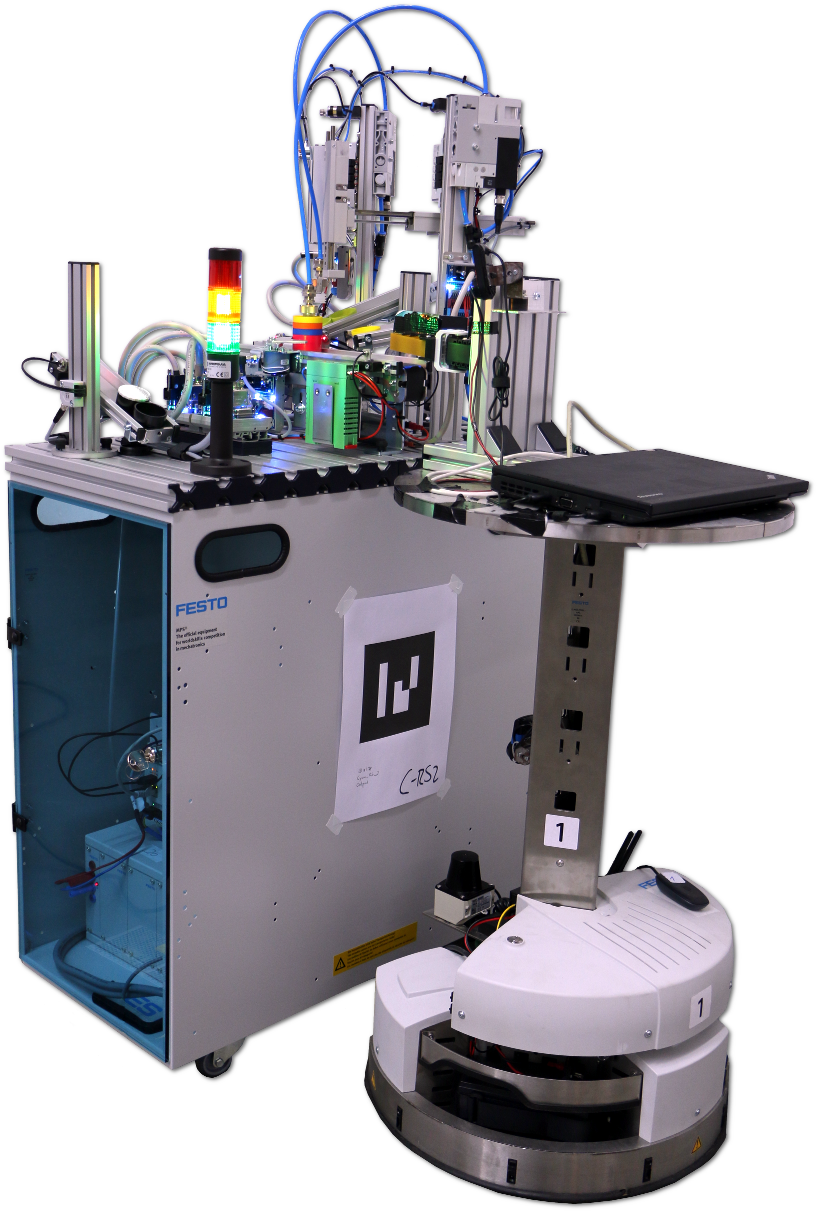
\includegraphics[width=0.5\textwidth]{img/rcll}
    \caption{Robot and MPS used in the RCLL}
    \label{fig:rcll}
  \end{minipage}
\quad
\begin{minipage}[b]{0.5\linewidth}
  \includegraphics[scale=0.45]{pics/production_chain}
  \caption[LLSF Production Chain]{LLSF Production Chain~\cite{LLSFRules}}
  \label{fig:llsf_chain}
\end{minipage}
\end{figure}

\todo[inline]{League, robotino}
%
The \textit{RoboCup Logistics League (RCLL)}\footnote{RoboCup
  Logistics League website: \url{http://www.robocup-logistics.org}},
previously LLSF, is a industry-oriented competition within RoboCup.
It tackles the problem of production logistics in a smart factory
where mobile robots have to plan, execute, and optimize the material
and production flow between machines to produce and deliver products
according to dynamic orders. Competing teams deploy a group of up to
three robots which have to autonomously build ordered products by
interacting with \textit{Modular Production Machines (MPS)} and
transporting workpieces between these machines.


%% received increasing attention. In 2012, the new industry-oriented
%% RoboCup Logistics League (RCLL, previously LLSF), was founded to
%% tackle the problem of production logistics. Groups of up to three
%% robots have to plan, execute, and optimize the material flow in a
%% smart factory scenario and deliver products according to dynamic
%% orders. Therefore, the challenge consists of creating and adjusting a
%% production schedule and coordinate the group of robots. We describe
%% the rules of 2014, to which this paper applies.
%% \begin{figure}[t]
%%   % when aligned at bottom:
%%   %\vspace{-3.8mm}
%%   \includegraphics[width=\linewidth,trim=0pt 140pt 0pt 27pt,clip]{figures/rc2014-finale-production.jpg}
%%   \caption{Carologistics (three Robotino 2 with laptops on top) and
%%     BavarianBendingUnits (two Robotino 3) during the LLSF finals at
%%     RoboCup 2014.}
%% \label{fig:rc2014-finale}
%% \vspace*{-2ex}
%% \end{figure}

%% \begin{figure}[b]
%%   \vspace{-3mm}
%%   \centering
    
%%   \tikzstyle{M}=[rectangle, draw=blue!50, thick, fill=blue!20, text width=2em,align=center, rounded corners=2pt, 
%%   minimum height=1.5em,inner sep=2pt]
%%   % 
%%   \tikzstyle{P}=[draw=orange, thick, circle,fill=orange!20, minimum height=1.5em,inner sep=2pt]
%%   \tikzstyle{FP}=[draw=orange, thick, circle,fill=red!20, minimum height=1.5em,inner sep=2pt]
%%   \tikzstyle{D}=[thick, level distance=1.2cm,sibling distance=0.8cm,draw=orange!80]

%%   \begin{tikzpicture}[D]
%%     \node [FP] (P) {\scriptsize $P_{1}$} [grow=left]
%%     child {
%%       node [M] (M3) {\scriptsize $T_3$}
%%       child { % -> S2
%%         node [P] (S2) {\scriptsize $S_2$}
%%         child { % -> S1
%%           node [M] (S1-M2) {\scriptsize $T_2$}
%%           child {
%%             node [P] (S2-S1) {\scriptsize $S_1$}
%%             child {
%%               node [M] (S2-S1-M1) {\scriptsize $T_1$}
%%               child {node [P] (S2-S1-S0) {\scriptsize $S_0$}}
%%             }
%%           }
%%           child {
%%             node [P] (S2-S0) {\scriptsize $S_0$}
%%           }
%%         }
%%       }
%%       child {
%%         node [P] (S0) {\scriptsize $S_0$}
%%       }
%%       child {
%%         node [P] (S1) {\scriptsize $S_1$}
%%         child {
%%           node [M] (S1-M1) {\scriptsize $T_1$}
%%           child {node [P] (S1-S0) {\scriptsize $S_0$}}
%%         }
%%       }
%%     };
%%   \end{tikzpicture}

%%   \caption{Production Chains for the most complex product of the RCLL 2014.}
%%   \label{fig:production-diagram}  
%% \end{figure}

%% \subsection{RoboCup Logistics League 2014}
%% The RCLL 2014 competition takes place on a field of \SI{11.2 x
%%   5.6}{\metre} (Fig.~\ref{fig:rc2014-finale}). Two teams are playing
%% at the same time competing for points by
%% fulfilling orders in time coping with robots of the other team.  Each
%% team has an exclusive input storage (blue areas) and delivery zone
%% (green area in figure \ref{fig:rc2014-finale}). Machines are
%% represented by RFID-readers with signal lights on top indicating the
%% machine state.  At the beginning all pucks (representing the products)
%% have the raw material state $S_0$, are in the input storage, and can
%% be refined (through several stages) to final products using the
%% production machines. These machines are assigned a type randomly at
%% the start of a match which determines what inputs are required and
%% what output will be produced, and how long this conversion will
%% take~\cite{LLSF-Sim}. The production tree for a complex product is
%% shown in \reffig{fig:production-diagram}. Orange circles denote input
%% products in a certain stage. One or more are fed into a machine (blue
%% boxes) and yield a certain output. Eventually, this leads to a
%% finished product (red circle). This must then be taken to the active
%% gate in the delivery zone. Machines may be down for a limited time to
%% simulate machine maintenance or faults.

%% The game is controlled by the \emph{referee box} (refbox), a software
%% component which keeps track of puck states, instructs the light
%% signals, and posts orders to the teams~\cite{LLSF2014}.  After the
%% game is started, no manual interference is allowed, robots receive
%% instructions only from the refbox. Teams are awarded with points for
%% producing complex products, delivering ordered products, and
%% recycling.
%% % The refbox can be seen as a higher-level production
%% %planning entity as used in industry, e.g.  ERP or MES-Systems.

%% In 2015, the RCLL introduces physical processing stations which
%% perform actual product modifications~\cite{LLSF2014} by stacking up
%% base products, colored rings, and caps. This also means a vastly
%% increased number of product variants that can be produced. Up from
%% three types to several hundreds. This makes RCLL also very
%% interesting from a planning and scheduling point of view as pointed
%% out in \cite{RCLL-Planning}.

\subsubsection{@Home League}
\todo[inline]{League, Ceasar}

%% The RoboCup@Home league is a
%% competition about service robots. The robots have to assist humans in
%% a domestic environment. There are a variety of tasks, such as
%% following a human, serving drinks and handling emergency
%% situations. Especially important in this league are the technical and
%% open challenge. Here, the teams can present their own ideas and how
%% the robot implements them.

\subsection{Fawkes Robot Software Framework}
\label{sec:fawkes}
%% \begin{itemize}
%% \item Component based approach
%% \item Blackboard
%% \item Comparison to ROS
%% \end{itemize}


\subsection{Planners and Reasoners}
\label{sec:planners}
\begin{itemize}
\item CLIPS
\item PDDL
\item Golog
\item MoveIt
\end{itemize}
\subsection{MongoDB}
\label{sec:mongodb}
\begin{itemize}
\item MongoDB
\item Query Language
\item Comparison to using CLIPS, KnowRob
\item Comparison to other DBs (SQL, Graph DBs, other Document DBs)
\end{itemize}

\section{Related Work}
\label{sec:related}
\subsection{KnowRob}
\label{sec:knowrob}
\begin{itemize}
\item Common sense Resoning
\item Concepts Ontologies, Triple Store, Virtual Knowledge base
\item Prolog implementation
\item Pro/Contra
\end{itemize}
\subsection{MongoDB Logging}
\label{sec:mongo-logging}
\subsection{More}
\todo[inline]{More}
\begin{itemize}
\item Blackboard
\item RoboEarth
\item Robot Memory... Robot Databases... Robot Knowledge Storage...
\end{itemize}


\section{Approach}
\label{sec:approach}
\subsection{Goals}
\label{sec:goals}
\begin{itemize}
\item Same worldmodel for reasoners/planners
\item Distributed for robot team
\item Long time storage (persistent, different kinds of long time knowledge, decay?)
\item Triggers
\item Interrupt storage?
\item Beliefs/Confidences?
\item Versatility (virtual knowledge base)
\item Temporal/Spatial grounding
\item Common sense knowledge
\end{itemize}
\subsection{Architecture}
\label{sec:arch}
\begin{itemize}
\item Data representation
\item Component interactions (diagram)
\item Data acquisition
\end{itemize}


\subsection{Implementation}
\label{sec:impl}
\subsubsection{Robot Memory}
\label{sec:impl-memory}
\begin{itemize}
\item Data Representation
\item MongoDB query language
\item Trigger
\item Multi-robot synchronization
\end{itemize}
\subsubsection{Planner/Reasoner}
\label{sec:impl-planner}
\begin{itemize}
\item Example for using the Robot Memory
\item Queries/Register Triggers
\item Build initial domain
\item When to replan
\end{itemize}

\subsection{Evaluation}
\label{sec:eval}
\subsubsection{Application}
\label{sec:eval-apl}
\begin{itemize}
\item RCLL PDDL-CLIPS
\item RCLL between bots
\item @Home
\end{itemize}
\subsubsection{Efficiency-Scalability}
\subsubsection{Expressiveness}
\subsubsection{Versatility}
\subsubsection{Software development expandability, interfacing}
\subsection{Schedule}
\begin{itemize}
\item Timetable
\end{itemize}

\section{Summery}
\label{sec:summery}
\begin{itemize}
\item Challenges
\item Impact
\end{itemize}


\bibliographystyle{plain}
\bibliography{../references}

\end{document}
